\chapter{The Artificial Neural Network} % (fold)
\label{cha:the_artificial_neural_network}
	In this first Chapter, we provide some informations about the Artificial Neural Network, i.e. a fully
	connected Multilayer Perceptron, we implemented from scratch. We'll describe both the network's structure and
	the algorithm we used in order to make our network \textit{learn} from the data used during the testing and
	validation phases. Finally we'll present the loss function we have chosen for our network, and we'll provide
	and explanation on how it is differentiable. We'll use the notation proposed in \cite{Goodfellow-et-al-2016}.

	\section{The ANN's structure} % (fold)
	\label{sec:the_ann_s_structure}
		Since we have to write from scratch an \textit{Artificial Neural Network}, ANN for short, we have
		considered some alternatives before choosing the network's final structure. We agreed on a structure
		composed by:

		\begin{itemize}
			\item one \textit{input layer};
			\item two \textit{hidden layers};
			\item one \textit{output layer};
		\end{itemize}

		As convention, the number of units in the input layer is egual to the number
		of features of the dataset that is used for the learning, validation and testing phases. The two
		hidden layers contain, respectively, four and eight \textit{hidden neurons}, following the convention of
		putting an increasing series of powers of two as number of hidden units per layer. The number of neurons
		for the output layer depends on the kind of task the network is trying to fullfil. In the case of a
		\textit{classification task}, like the MONKS dataset \cite{Dua:2019}, we have decided to put one unit in
		the output layer, while in the case of a \textit{regression task}, like the CUP dataset, we have decided to
		put two units in the output layer. As we have seen studying the papers and books for gathering the
		necessary knowledge for the project, as \cite{Goodfellow-et-al-2016,haykin2009neural,mitchell1997machine},
		choosing to consider the network's structure as an \textit{hyperparameter}, that is, a variable, could
		lead to a series of difficult choices during the validation phase, so we have decided to fix the ANN
		structure to the one described for both the task we have to fullfil, changing only the number of units in
		the output layer from task to task. In figure \ref{fig:ann_structure} you can see our ANN's graph for
		the classification task.

		\begin{figure}
			\centering
			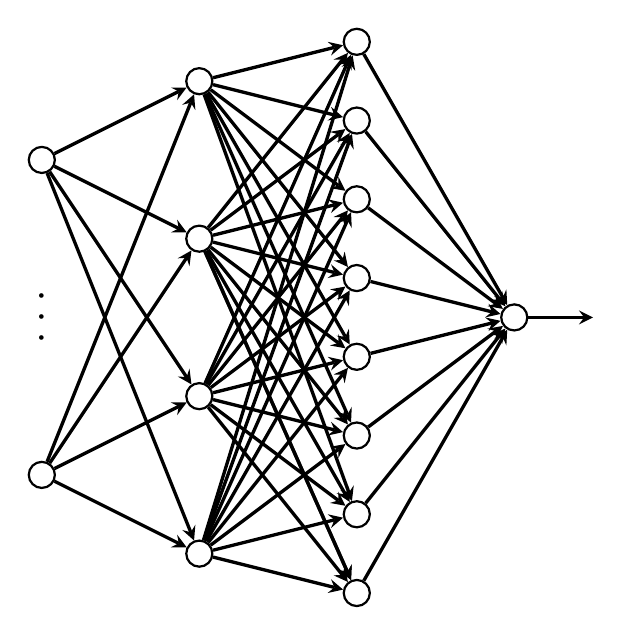
\begin{tikzpicture}
				\begin{scope}[every node/.style={circle,thick,draw}]
                    \node (A) at (-2,0) {};
                    \node (B) at (-2,-4) {};
                    \node (C) at (0,1) {};
                    \node (D) at (0, -1) {};
                    \node (E) at (0,-3) {};
                    \node (F) at (0,-5) {};
                    \node (G) at (2,1.5) {};
                    \node (H) at (2,0.5) {};
                    \node (I) at (2,-0.5) {};
                    \node (L) at (2,-1.5) {};
                    \node (M) at (2,-2.5) {};
                    \node (N) at (2,-3.5) {};
                    \node (O) at (2,-4.5) {};
                    \node (P) at (2,-5.5) {};
                    \node (Q) at (4,-2) {};
                \end{scope}

                \coordinate[right of=Q] (d1);

                \path (A) -- (B) node [black, font=\LARGE, midway, sloped] {$\dots$};

                \begin{scope}[>={stealth[black]},
                every edge/.style={draw=black,very thick}]
                    \path [->] (A) edge node {} (C);
                    \path [->] (A) edge node {} (D);
                    \path [->] (A) edge node {} (E);
                    \path [->] (A) edge node {} (F);
                    \path [->] (B) edge node {} (C);
                    \path [->] (B) edge node {} (D);
                    \path [->] (B) edge node {} (E);
                    \path [->] (B) edge node {} (F);

                    \path [->] (C) edge node {} (G);
                    \path [->] (C) edge node {} (H);
                    \path [->] (C) edge node {} (I);
                    \path [->] (C) edge node {} (L);
                    \path [->] (C) edge node {} (M);
                    \path [->] (C) edge node {} (N);
                    \path [->] (C) edge node {} (O);
                    \path [->] (D) edge node {} (P);
                    \path [->] (D) edge node {} (G);
                    \path [->] (D) edge node {} (H);
                    \path [->] (D) edge node {} (I);
                    \path [->] (D) edge node {} (L);
                    \path [->] (D) edge node {} (M);
                    \path [->] (D) edge node {} (N);
                    \path [->] (D) edge node {} (O);
                    \path [->] (D) edge node {} (P);
                    \path [->] (E) edge node {} (G);
                    \path [->] (E) edge node {} (H);
                    \path [->] (E) edge node {} (I);
                    \path [->] (E) edge node {} (L);
                    \path [->] (E) edge node {} (M);
                    \path [->] (E) edge node {} (N);
                    \path [->] (E) edge node {} (O);
                    \path [->] (E) edge node {} (P);
                    \path [->] (F) edge node {} (G);
                    \path [->] (F) edge node {} (H);
                    \path [->] (F) edge node {} (I);
                    \path [->] (F) edge node {} (L);
                    \path [->] (F) edge node {} (M);
                    \path [->] (F) edge node {} (N);
                    \path [->] (F) edge node {} (O);
                    \path [->] (F) edge node {} (P);

                    \path [->] (G) edge node {} (Q);
                    \path [->] (H) edge node {} (Q);
                    \path [->] (I) edge node {} (Q);
                    \path [->] (L) edge node {} (Q);
                    \path [->] (M) edge node {} (Q);
                    \path [->] (N) edge node {} (Q);
                    \path [->] (O) edge node {} (Q);
                    \path [->] (P) edge node {} (Q);

                    \path [->] (Q) edge node {} (d1);
                \end{scope}
			\end{tikzpicture}
			\caption{The ANN's structure for the classification task, the majority of the input nodes are
			omitted because they vary from dataset to dataset.}
			\label{fig:ann_structure}
		\end{figure}
	% section the_ann_s_structure (end)

	\section{Initializing the Network} % (fold)
	\label{sec:initializing_the_network}
		As we know from \cite{Goodfellow-et-al-2016,haykin2009neural,mitchell1997machine}, an ANN is composed by
		a set of weights $\mathbf{W}_{i}$, and a set of biases $\mathbf{b}_{i}$,
		$i \in \{ 1, \ \ldots \ , \ l \}$, with $l$ representing the ANN's number of layers. Although it is common
		practice to initialized the network's weights and biases to random, small, values, we have decided to
		follow the \textit{normalized initialization}, as described in
		\cite{Glorot10understandingthe,Goodfellow-et-al-2016}, which defines the initial values for the weights
		and the biases for each layer in the uniform distribution taken in the range

		\begin{equation*}
		    W \sim U \left [ -\frac{\sqrt{6}}{\sqrt{m + n}}, \ \frac{\sqrt{6}}{\sqrt{m + n}} \right ]
		\end{equation*}

		with $m$ and $n$, representing the number of inputs and outputs for each layer. This heuristic is
		designed to compromise between the goal of initializing all layers to have the same activation variance
		and the goal of initializing all layers to have the same gradient variance. The formula is derived using
		the assumption that the network consists only of a chain of matrix multiplications, with no
		nonlinearities. Other than this kind of initialization, we also make available the standard
		\textit{random initialization} for creating a network, described at the beginning of this \S, which
		initialize the weights and the biases for each layer in the uniform distribution taken in the range

		\begin{equation*}
		    W \sim U \left [ - 0.7, \ 0.7 \right ].
		\end{equation*}
	% section initializing_the_network (end)

	\section{The back-propagation algorithm} % (fold)
	\label{sec:the_back-propagation_algorithm}
		The learning procedure for our ANN essentialy consist in two distinct phases:

		\begin{enumerate}
			\item compute the network's \textit{gradient}, that is, the derivative of the cost function
			$\nabla_{\theta} J(\theta)$, with $\theta$ representing the ANN's hyperparameters, with respect to
			every network's unit using the well known \textit{back-propagation algorithm}, described by
            algorithm \ref{alg:forward_propagation} and \ref{alg:backward_propagation};
			\item optimize the information gathered during the first phase using a distinct optimizer, chosen
			among the \textit{Stochastic Gradient Descent} and the \textit{Conjugate Gradient Method}, as
			described in Chapter \ref{cha:optimizers};
		\end{enumerate}

		For computing the gradient we have chosen to use
		the well known \textit{backpropagation algorithm}, firstly introduced in \cite{10028086174} and described
		in \cite{Goodfellow-et-al-2016,haykin2009neural,mitchell1997machine}. This algorithm is
		also composed by two phases, a first phase, that is, the \textit{forward propagation}, in which the
		feature vector $\mathbf{x}$ given in input has to flow from the input layer through the hidden layers and,
		finally, the output layer, giving the approximation $\hat{\mathbf{y}}$ as output, and a second one, that
		is, the \textit{back-propagation}, which allows the information to flow backward through the network in
		order to compute the gradient by applying the Chain Rule of Calculus, that is, a technique for computing the
		derivative of a composition of functions.

		\begin{algorithm}[H]
			\caption{Forward propagation through a typical (deep) neural network and the computation of the cost
			function. Here $L(\hat{\mathbf{y}}, \mathbf{y})$ represents the loss function evaluated using both
			$\mathbf{y}$ and $\hat{\mathbf{y}}$ as inputs, more details about that will be provided in
			\S \ref{sec:the_loss_function}. The function $f$ applied on line $5$ represents
			the layer's \textit{activation function}, while $\lambda \Omega(\theta)$ represents the
			network's regularization term, with $\theta$ representing the ANN's hyperparameters.}
			\label{alg:forward_propagation}
			\begin{algorithmic}[1]
				\Procedure{Forward propagation}{$l$, $\mathbf{W}_{i} \ i \in \{ 1, \ldots, l \}$,
				$\mathbf{b}_{i} \ i \in \{ 1, \ldots, l \}$, $\mathbf{x}$, $\mathbf{y}$}
					\State $\mathbf{h}_{0} = \mathbf{x}$
					\For{$k = 1, \ldots, l$}
						\State $\mathbf{a}_{k} = \mathbf{b}_{k} + \mathbf{W}_{k}\mathbf{h}_{k - 1}$
						\State $\mathbf{h}_{k} = f(\mathbf{a}_{k})$
					\EndFor
					\State $\hat{\mathbf{y}} = \mathbf{h}_{l}$
					\State $J = L(\hat{\mathbf{y}}, \mathbf{y}) + \lambda \Omega(\theta)$
				\EndProcedure
			\end{algorithmic}
		\end{algorithm}

		Since each one of the ANN's layers has its own
		\textit{activation function}, that is, a function that has to be applyied to the output of every layer's
		neuron, it is particularly usefull to think of the ANN like a composition of functions, and, for this
		reason, the Chain Rule of Calculus play a decisive role in the gradient's computation by back-propagation.
		It is import to note that with the term back-propagation we mean
		only the method for computing the gradient, not the whole learning algorithm. We now provide the
		pseudocode for the forward propagation and the back-propagation phases, as shown in algorithms
		\ref{alg:forward_propagation} and \ref{alg:backward_propagation}.

		\begin{algorithm}[H]
			\caption{Backward computation for the (deep) neural network of algorithm
			\ref{alg:forward_propagation}. Here, the $\odot$ symbol represents the element-wise
			(Hadamard) product, while $\nabla_{\hat{\mathbf{y}}}J =
			\nabla_{\hat{\mathbf{y}}}L(\hat{\mathbf{y}}, \mathbf{y})$ represents the gradient of the loss
			function computed with respect to the output $\hat{\mathbf{y}}$. $\nabla_{\mathbf{b}_{k}}J$,
			$\nabla_{\mathbf{W}_{k}}J$ and $\nabla_{\mathbf{h}_{k - 1}}J$ represents the gradient of the
			loss function computed with respect to, respectively, $\mathbf{b}_{k}$, $\mathbf{W}_{k}$ and
			$\mathbf{h}_{k - 1}$, and finally $\nabla_{\mathbf{b}_{k}} \Omega(\theta)$ and
			$\nabla_{\mathbf{W}_{k}} \Omega(\theta)$ represents the gradient of the ANN's hyperparameters computed
			with respect to, respectively, $\mathbf{b}_{k}$ and $\mathbf{W}_{k}$.}
			\label{alg:backward_propagation}
			\begin{algorithmic}[1]
				\Procedure{Backward propagation}{}
					\State $\mathbf{g} \leftarrow \nabla_{\hat{\mathbf{y}}}J = \nabla_{\hat{\mathbf{y}}}
					L(\hat{\mathbf{y}}, \mathbf{y})$
					\For{$k = l, l - 1, \ldots, 1$}
						\State $\mathbf{g} \leftarrow \nabla_{\mathbf{a}_{k}}J = \mathbf{g} \ \odot \
						f'(\mathbf{a}_{k})$
						\State $\nabla_{\mathbf{b}_{k}}J = \mathbf{g} \ + \ \lambda \nabla_{\mathbf{b}_{k}}
						\Omega(\theta)$
						\State $\nabla_{\mathbf{W}_{k}}J = \mathbf{g}\mathbf{h}_{k - 1}^{T} \ + \ \lambda
						\nabla_{\mathbf{W}_{k}} \Omega(\theta)$
						\State $\mathbf{g} = \nabla_{\mathbf{h}_{k - 1}}J = \mathbf{W}_{k}^{T}\mathbf{g}$
					\EndFor
				\EndProcedure
			\end{algorithmic}
		\end{algorithm}
	% section the_back-propagation_algorithm (end)

	\section{The activation functions} % (fold)
	\label{sec:the_activation_functions}
		As we have mentioned in \S \ref{sec:the_back-propagation_algorithm}, each one of the ANN's layers
		has an \textit{activation function}, that is, a function that is applied to $\mathbf{a}_{k}$ in order to
		obtain $\mathbf{h}_k$, with $k \in \{1,\ldots,l\}$. We can say that an activation function of a node
		defines the output of that node, and maps $\mathbf{a}_{k}$ into the desired range. For being chosen as
		an activation function, a function has to possess a series of properties, such as

		\begin{itemize}
			\item \textit{nonlinearity}: when the activation function is non-linear, then a two-layer neural
			network can be proven to be a universal function approximator;
			\item \textit{range}: when the range of the activation function is finite, gradient-based training
			methods, such as the ones described in chapter \ref{cha:optimizers}, tend to be more stable, because
			pattern presentations significantly affect only limited weights;
			\item \textit{continuously differentiable}: since the functions have to be envolved in the Chain Rule
			of Calculus during the gradient's computation in the back-propagation algorithm;
		\end{itemize}

		There are many functions that can be used as activation functions for an ANN; we have chosen to utilize the
		well known \textit{logistic function}, i.e. the \textit{sigmoid function}, which is computed as

		\begin{align*}
		    &f(x) = \sigma(x) = \frac{1}{1 + e^{-x}} \\
		    &f'(x) = \sigma'(x) = f(x)(1 - f(x)),
		\end{align*}

		and is defined in the range $\left ( 0,\ 1 \right )$. As introduced in \S
        \ref{sec:the_back-propagation_algorithm}, we can think the ANN as a \textit{composition} of activation
        functions, and, since we have stated that each one of the network's layers uses the logistic function as
        activation function, we can represent the ANN as

        \begin{equation*}
            \sigma_l \ \circ \ \sigma_{l - 1} \ \circ \ \cdots \ \circ \ \sigma_1
        \end{equation*}

        with $l$ representing the total number of layers in the network and $\sigma$ representing the logistic
        function.

	% section the_activation_functions (end)

	\section{The Loss function} % (fold)
	\label{sec:the_loss_function}
		It \S \ref{sec:the_back-propagation_algorithm} we have referred to the \textit{Loss function} as to a
		function that takes as input the ANN's output vector $\hat{\mathbf{y}}$ and the \textit{ground truth}
		vector $\mathbf{y}$, that is, the vector containing the desired output for the network. But what
        essentially is a Loss function? As a matter of fact, the Loss function can be considered like
		one way of measuring the performance, or equivalently the error, of the model that utilizes it, an ANN in
		this case. There are various types of Loss functions, for our network we have decided to use a well
		known function: the \textit{Mean Squared Error}, MSE for short, for both the classification and the
        regression tasks. The MSE is obtained with the formula

		\begin{equation*}
		\label{mse}
		    \text{MSE} = \frac{1}{m}\sum_{i = 1}^{m}\left ( \hat{\mathbf{y}} - \mathbf{y} \right )^{2}_{i},
		\end{equation*}

		where $m$ represents the number of samples for which we computed the output $\hat{\mathbf{y}}$. We can
        represent this functions also as a composition of the square function and the Euclidean norm by writing
        the latter formula as

        \begin{equation*}
            \text{MSE} = \frac{1}{m}|| \hat{\mathbf{y}} - \mathbf{y} ||^2_2 .
        \end{equation*}

        Since this formula is used for computing the performances of our models, our primary goal is to minimize its
		output as much as possible by computing the gradient during the backward propagation step of the
		back-propagation algorithm, as described in \S \ref{sec:the_back-propagation_algorithm}. Of course,
        in order to do so, it must be a \textit{differentiable} function. The gradient for the MSE with respect to
		$\hat{\mathbf{y}}$ is defined as:

		\begin{equation*}
		     \nabla_{\hat{\mathbf{y}}}\text{MSE}\left(\hat{\mathbf{y}},\ \mathbf{y}\right) =
		     \hat{\mathbf{y}} - \mathbf{y}.
		\end{equation*}

        \subsection{Properties of the Loss function} % (fold)
        \label{sub:properties_of_the_loss_function}
            Here we discuss the relevant properties of the Loss function we have chosen for our model.

            \begin{itemize}
                \item \textbf{Continuity}. As we introduced in this section, our Loss function is a function in
                two variables, $\hat{\mathbf{y}}$ and $\mathbf{y}$, respectively. A function $f$ in two variables
                is L-Lipschitz continuous if there exists a constant L such that

                \begin{equation*}
                    || f(\mathbf{x}_1, \mathbf{y}_1) - f(\mathbf{x}_2, \mathbf{y}_2) || \le L(|| \mathbf{x}_1 -
                    \mathbf{x}_2|| + || \mathbf{y}_1 - \mathbf{y}_2||) \quad \forall (\mathbf{x}_1, \mathbf{y_1}),
                    (\mathbf{x}_2, \mathbf{y_2}) \ \in \ \mathbf{dom} \ f.
                \end{equation*}

                Being the MSE a composition of the square function and the Euclidean norm, because of the squaring,
                the function is Lipschitz continuous only if we restrict its domain to a bounded set. Since, as
                described in \S \ref{sec:the_activation_functions}, each network's layer uses the sigmoid
                function, which is a squashing function that bounds every layer's output in the range
                $\left ( 0,\ 1 \right )$, the MSE can be considered as a continous function.
                \item \textbf{Differentiability}. Again, being the sigmoid function the one used by the ANN,
                and since the sigmoid function is continuously differentiable with bounded Lipschitz continuous
                derivative, we can consider the MSE as a differentiable function, being the network a
                composition of continuously differentiable functions. If we restrict the weights to a
                bounded set and we adopt only activation functions with Lipschitz derivative, the
                gradient of our loss functions is Lipschitz continuous, since it is a product of bounded
                Lipschitz continuous functions. In section \S \ref{sec:initializing_the_network} we
                described the method we have used to initialize our ANN's weights, this method is
                guaranteed to restrict the weights to a bounded set, furthermore, the properties of
                the logistic function permit the gradient of our loss functions to be Lipschitz
                continuous.
                % Futhermore, a differentiable
                % function is said to have an L-Lipschitz continuous gradient if, for some $L>0$ holds:

                % \begin{equation*}
                %     || \nabla f(\mathbf{x}) - \nabla f(\mathbf{y}) || \le L(|| \mathbf{x} - \mathbf{y}||)
                %     \quad \forall (\mathbf{x}, \mathbf{y}), \ \in \ \mathbf{dom} \ f.
                % \end{equation*}

                % Since the Loss function is bounded in the interval dectated by the logistic function, we
                % can say that the gradient of the function is also bounded in the same interval, so the
                % MSE has an L-Lipschitz continuous gradient.
                \item \textbf{Convexity}. We recall that, for $h \ : \ \mathbb{R}^k \to \mathbb{R}$, $g_i \ : \
                \mathbb{R}^n \to \mathbb{R}$, the function:

                \begin{equation*}
                    f(\mathbf{x}) = h(g_1(\mathbf{x}), \ldots, g_k(\mathbf{x}))
                \end{equation*}

                is convex if $\mathbf{dom} \ h = \mathbb{R}^k$, $\mathbf{dom} \ g = \mathbb{R}^n$, $h$ is convex,
                $h$ is non-decreasing in each argument and $g_i$ are convex. For the aforesaid result, the squared
                Euclidean distance is convex, as any distance is non-negative and the square function is convex and
                increasing for non-negative values; however, when composed with another function it may not be
                convex. The functions that compose the network, that is, the sigmoid functions, are not convex
                functions, hence we can conclude that, for our network, the MSE is a not convex function.
            \end{itemize}

        % subsection properties_of_the_loss_function (end)

% chapter the_artificial_neural_network (end)
